%\documentclass[a4paper,10pt]{article}
\documentclass[10pt,foldmark]{leaflet}
\renewcommand*\foldmarkrule{.3mm}
\renewcommand*\foldmarklength{5mm}
\usepackage{qrcode}
\usepackage{amsmath}
\usepackage[T1]{fontenc}
\usepackage{textcomp}
\usepackage{mathptmx}
\usepackage[scaled=0.9]{helvet}
\usepackage[utf8]{inputenc}
\usepackage{graphicx}

%opening
\title{S.D.S. TH7: Seven Channel Thermocouple  Pi Hat}
\author{Scientific Data Systems}
\begin{document}
%\thispagestyle{empty} % get rid of page number does not work
\pagenumbering{gobble}
\maketitle
% \begin{abstract}
% This leaflet describes the TH7 generic thermocouple reader pi-hat/PCB for the raspberry pi.
% \end{abstract}

\begin{figure}
 \centering
 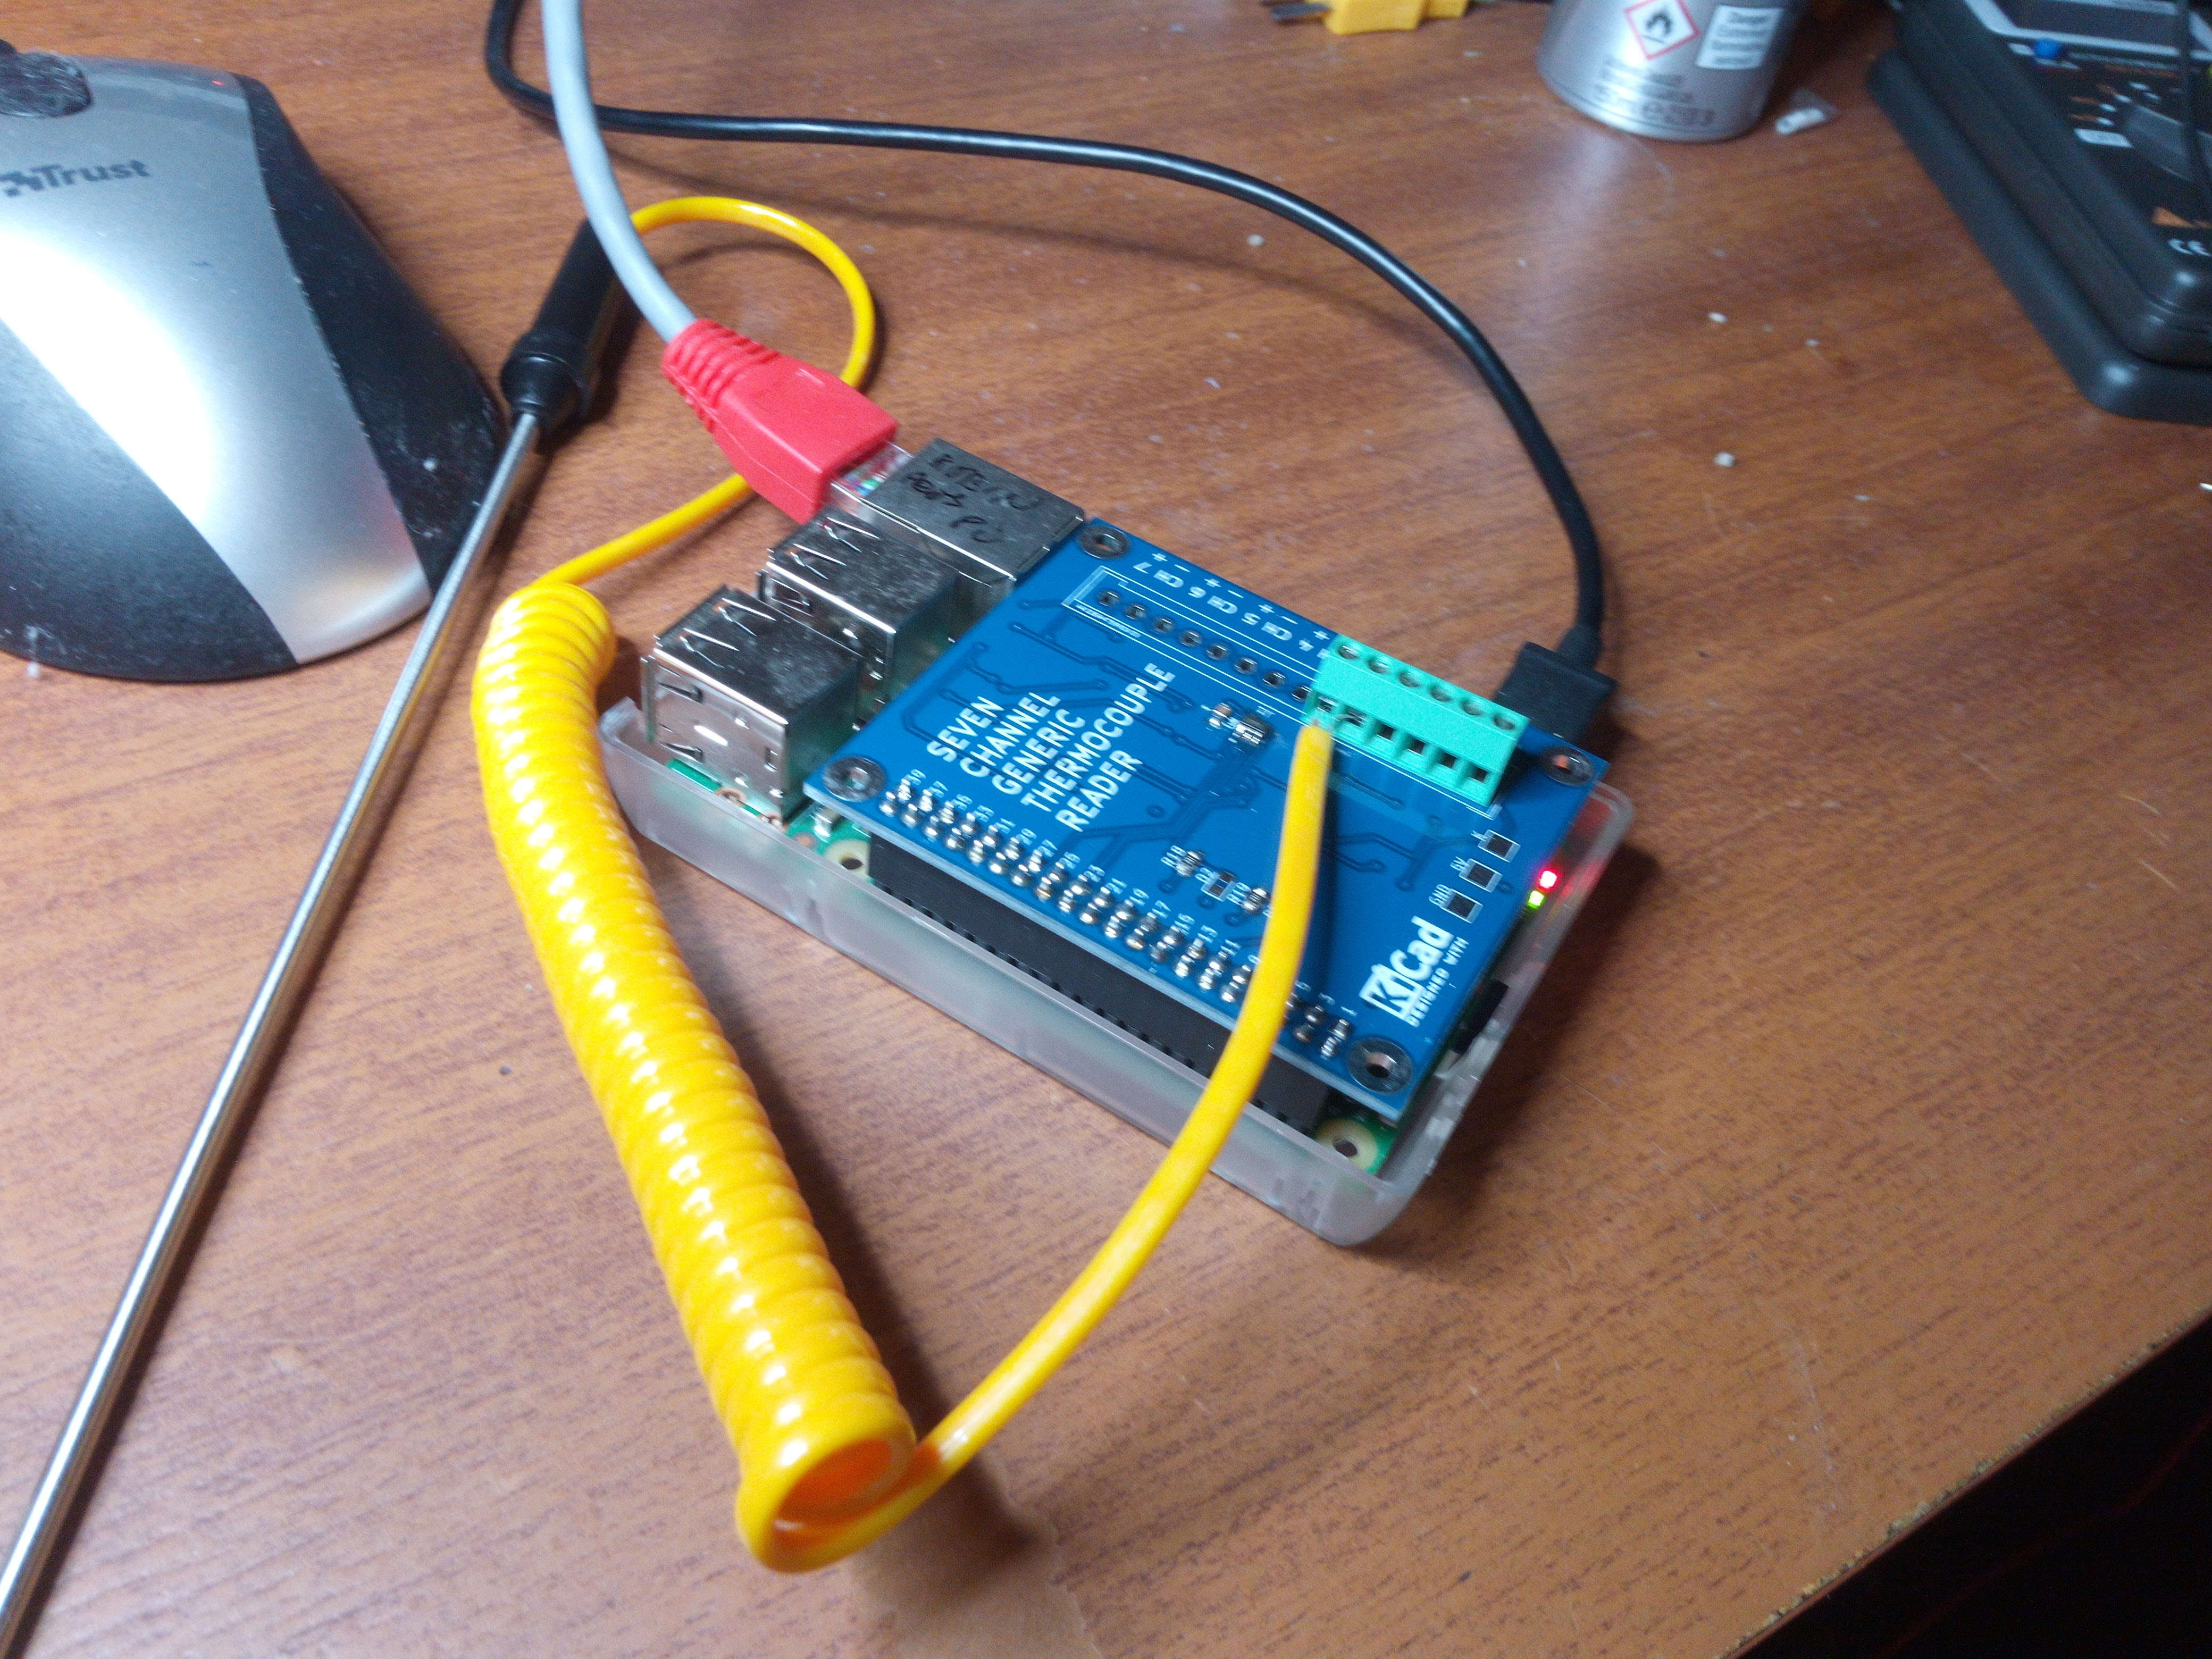
\includegraphics[width=200pt]{./TH7_0p4_IMG_20181010_184556D.jpg}
 % TH7_0p4_IMG_20181010_184556D.jpg: 0x0 pixel, 300dpi, 0.00x0.00 cm, bb=
 \caption{TH7 with a `k' type probe fitted.}
 \label{fig:th7}
\end{figure}



\section{TH7 description}
The TH7 is a raspbery pi hat   that
provides seven thermocouple inputs(see figure~\ref{fig:th7}). This mean seven different temperatures can be read
simultaneously. Its possible uses are 
logging/monitoring and control of temperature sensitive processes.
%
With on board PCB temperature measurement
it provides full Cold~Junction~Compensation (CJC).
Uncalibrated the TH7 gives a typical accuracy of $\pm$ ${2}^{\circ} C$.
It also provides two user programmable LEDS and displays the supply voltage to the pi.
\clearpage
The TH7 is a generic thermocouple reader, and therefore should work with any thermocouple.
Software defines its micro-volt to temperature and cold~junction~compensation characteristics.
Software support has been written for the `k' type only currently.

%\clearpage
\subsection{Characteristics}
The TH7 offers:
\begin{itemize}
 \item Full cold junction compensation;
 \item Loss of/disconnection of thermocouple detection;
 \item Seven inputs;
 \item Uses the rasberry pi standard python SPI interface;
 \item Python coding examples \\ https://github.com/robin48gx/TH7;
 \item Two user Programmable LEDs;
 \item On chip PCB temperature measurement;
  \item Can be used as a general micro-volt reader with a $\approx -6000 \mu V \rightarrow 40000 \mu V$ range.
\end{itemize} 

\section{Instructions}
\subsection{Connection to terminal block}
Connect the thermocouples using the hital~tech connectors and ensure the wires make contact with the 
connector metal clamps (see figure~\ref{fig:con}).
\subsection{Conection to the device being measured}
Always apply insulation to the thermocouples (i.e. do not ground them).
Epoxy resin is often useful for gluing thermcouples to devices under long term temperature test.

\begin{figure}[h]
 \centering
 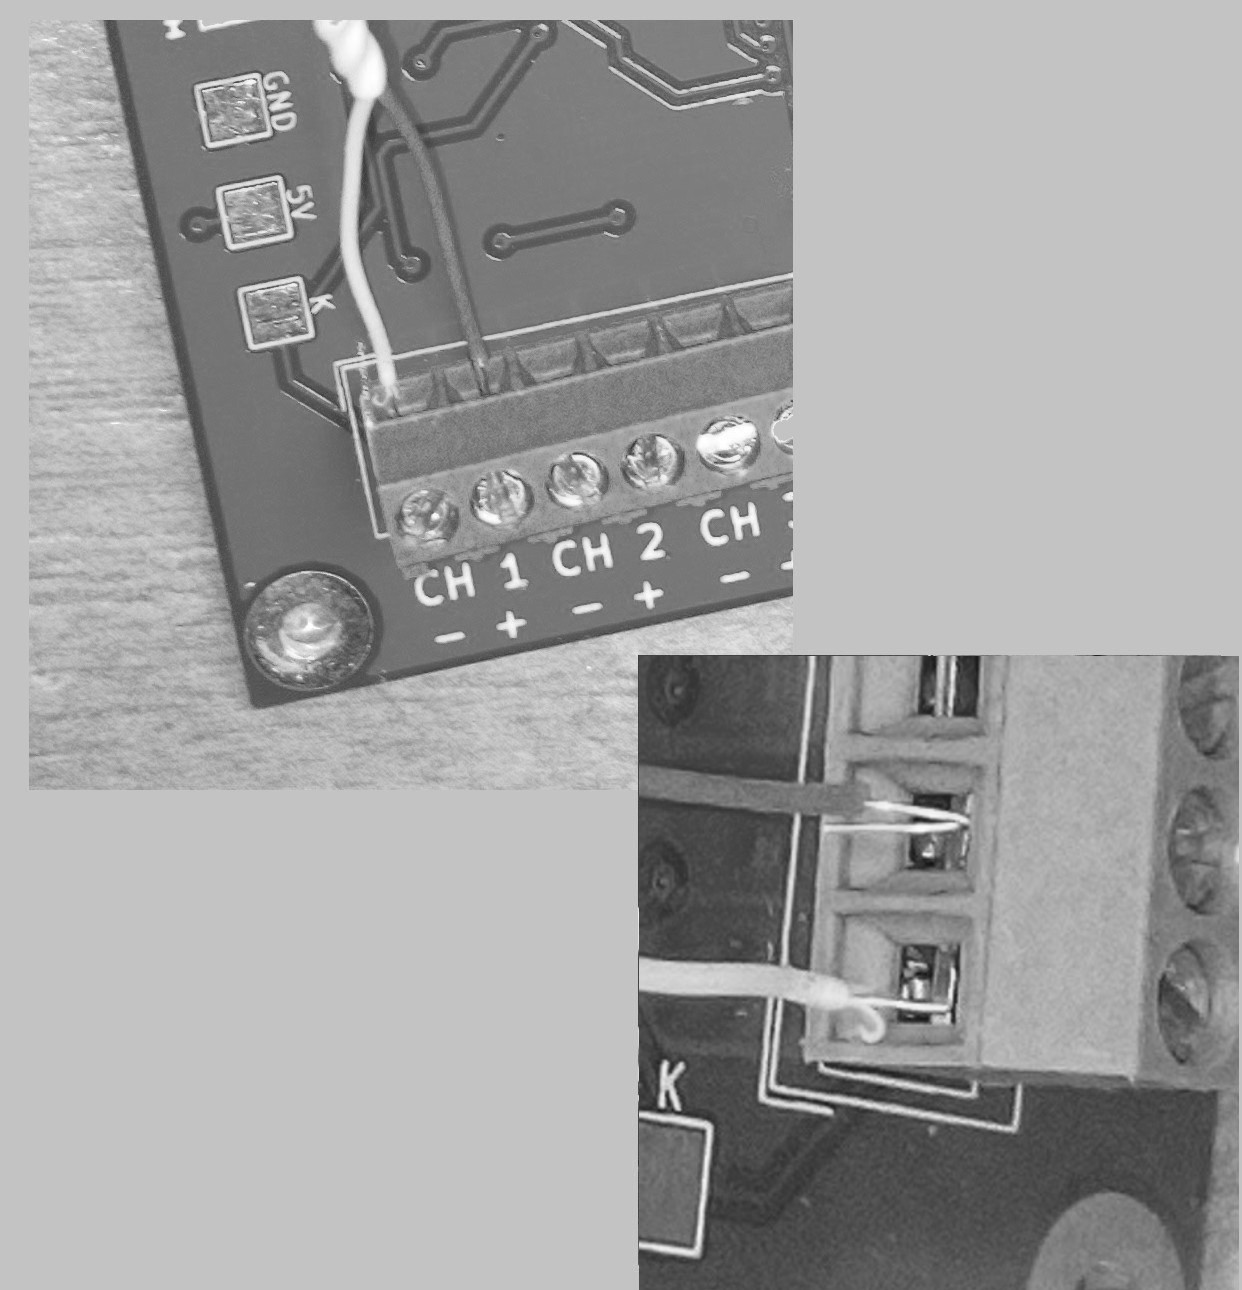
\includegraphics[width=200pt]{./wiring.jpg}
 % wiring.JPG: 0x0 pixel, 300dpi, 0.00x0.00 cm, bb=
 \caption{image shows wiring for European standard `k' type thermocouples Wiring (green is plus and the green and white is minus; other countries may use different colour schemes). 
 If the thermoucouple is inserted with incorrect polarity it will read incorrectly and temperature from it will be seen to go down when heat is applied to it.}
 \label{fig:con}
\end{figure}

\begin{figure}[h]
 \centering
 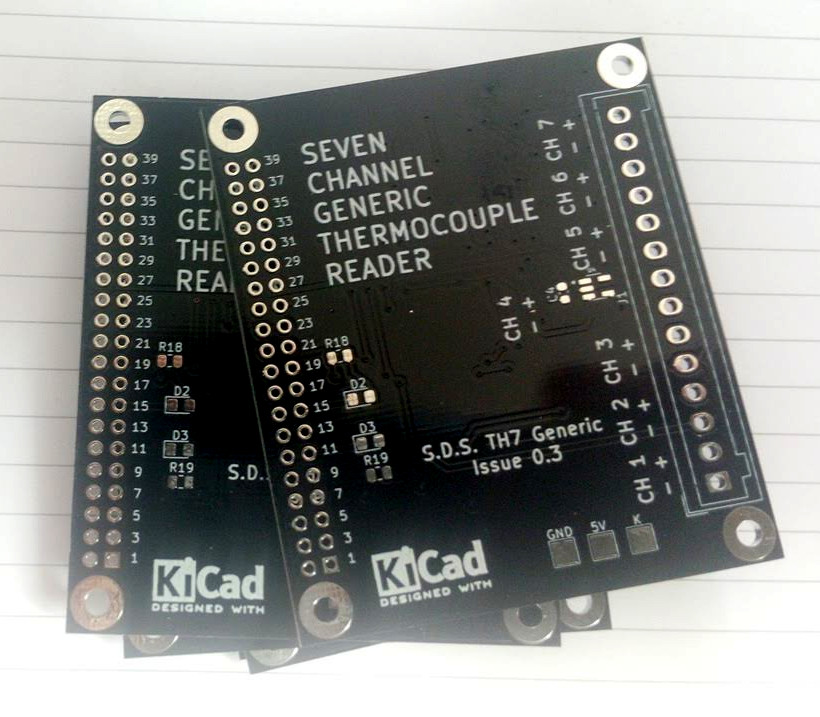
\includegraphics[width=156pt]{./TH7_0p3.jpg}
 % TH7_0p3.jpg: 0x0 pixel, 300dpi, 0.00x0.00 cm, bb=
 \caption{TH7 thermocouple interface PCB/pi~Hat}
 \label{fig:th7_2}
\end{figure}

\clearpage
\begin{figure}[ht]
 \centering
 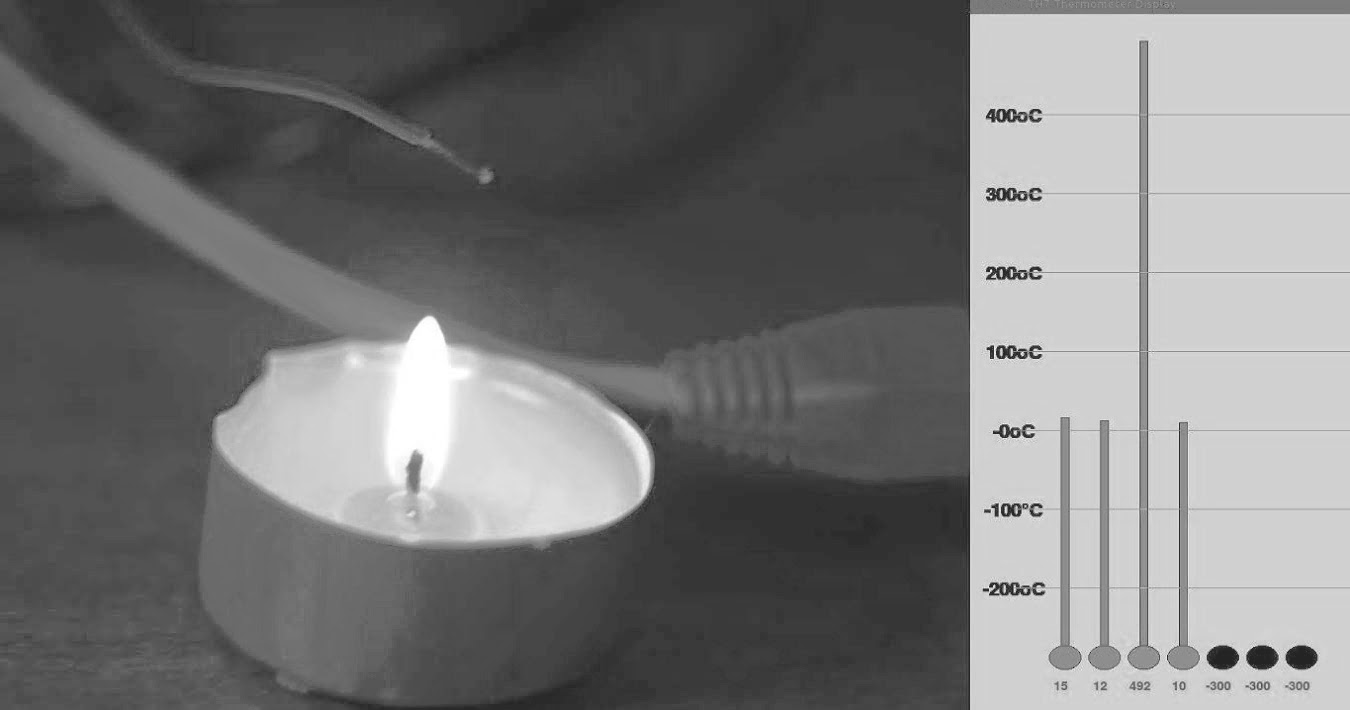
\includegraphics[width=200pt]{TH7_tea_light.jpg}
 % TH7_tea_light.JPG: 0x0 pixel, 300dpi, 0.00x0.00 cm, bb=
 \caption{Thermocouple over a tea light flame at circa ${500}^{\circ} C$.}
 \label{fig:pi}
\end{figure}
\mbox{}
\vfill

\qrcode[height=1in]{http://www.scientificdatasystems.co.uk}

\vspace{0.5cm}
Contact: info@scientificdatasystems.co.uk

\clearpage

\section{What Thermocouples are}

Thermocouples are two different types of metal wire welded together
at one end.
When there is a heat difference between two ends of the wire
the two metals produce a small voltage.
This is typically very small, for `k' type thermocouples for instance
this is about 40 millionths of a volt per Centigrade change in temperature.
%
This voltage is so small that ordinary voltage reading chips, Analogue to Digital Converters (ADC),  cannot easily read them
to any reasonable accuracy.
%
The small signal is usually amplified
to take it into the range that a computer chip can read it.
The TH7 has an amplifier that takes the small voltage and amplifies it by 100.
It can than be read into the raspberry pi where it can be converted into
a temperature reading with adequate accuracy.
Wikipedia has a good entry on thermocouples.
https://en.wikipedia.org/wiki/Thermocouple.
%as a qrcode, \qrcode[height=1in]{https://en.wikipedia.org/wiki/Thermocouple}

\subsection{Cold Junction Compensation}

The tables and equations to convert thermocouple voltage to
temperature all assume that the instrument end is at zero centigrade.

Because the voltage read at the TH7 input is not at zero centigrade (well not normally!)
the junction of the wires {\em at the connector block}  makes a thermocouple its-self, but in opposition to
the one at the measurement end. For instance, with a `k' type thermocouple
the volatge read at $25^\circ C$ would read around $1000 \mu V$ low!

The TH7 has a temperature measurement chip placed right by the terminal block for the thermocouple inputs.
By knowing this temperature, the TH7 works out what the missing voltage is
and adds it in before calculating the final temperature. This is commonly known as cold junction compensation.

\subsection{Using the TH7 as a micro-volt reader}

The TH7 can be used as a general micro-volt reader.
The voltage source must be floating i.e. not grounded.
A range of $\approx -6mV \rightarrow 40mV$ can be read.
\clearpage
\subsection{Pricing}

TH7 boards are currently available for 50 pounds each with a four week lead time.
\vspace{3.5cm}
%\clearpage
\mbox{}
\vfill
\qrcode[height=1in]{http://www.scientificdatasystems.co.uk}

\vspace{0.5cm}
Contact: info@scientificdatasystems.co.uk


\end{document}
